\documentclass[12pt, answers]{exam}
\usepackage[utf8]{inputenc}

\usepackage[margin=1in]{geometry}
\usepackage{amsmath,amssymb}
\usepackage{multicol}
\usepackage[]{graphicx}
\usepackage[]{bm}
\usepackage[]{nicefrac}
\usepackage[]{xcolor}

\newcommand{\class}{Physique non-linéaire}
\newcommand{\term}{Master 2}
\newcommand{\examnum}{Examen final}
\newcommand{\examdate}{Février 2021}
\newcommand{\timelimit}{120 Minutes}

\pagestyle{head}
\firstpageheader{}{}{}
\runningheader{\class}{\examnum\ - Page \thepage\ of \numpages}{\examdate}
\runningheadrule

\usepackage[]{tikz}

\begin{document}

\noindent
\begin{tabular*}{\textwidth}{l @{\extracolsep{\fill}} r @{\extracolsep{6pt}} l}
% \textbf{\class} & \textbf{Nom -- Prénom:} & \makebox[2in]{\hrulefill}\\
% \textbf{\term} &&\\
\textbf{\examnum} &&\\
\textbf{\examdate} &&
% \textbf{Time Limit: \timelimit} & Teaching Assistant & \makebox[2in]{\hrulefill}
\textbf{Durée: \timelimit} %&&
\end{tabular*}\\
\rule[2ex]{\textwidth}{2pt}

Ce sujet contient \numpages\ pages (en comptant la page de garde) et \numquestions\ exercices.\\
Le nombre total de point est de \numpoints.

\begin{center}
  Barême\\
  \bigskip
  \addpoints
  \gradetable[v][questions]
\end{center}

\noindent
\rule[2ex]{\textwidth}{2pt}

\begin{questions}

  \question[10] \textbf{Ferrer le poisson}
  \noaddpoints
  
  Considérons une population de poissons dont l'évolution au cours du temps peut être modélisée à l'aide de l'équation logistique suivante
  %
  \[
  \dfrac{dP}{dt} = r P \left( 1 - \dfrac{P}{N} \right)
  \]
  %
  où $P(t) \in \mathbb{R}$ est la population au temps $t$, $r > 0$ le taux de reproduction et $N > 0$ la population maximale pouvant être supportée par l'environnement.
  Dans la suite de cet exercice, nous nous intéresserons à l'influence de deux stratégies de pêche sur l'évolution de cette population de poissons.

  \textbf{Pêche constante}

  La première stratégie que nous allons considérer est celle d'un prélèvement constant sans prise en compte de l'état  courant de la population.
  Si l'on note par $H$ ce taux constant, alors notre modèle peut être écrit comme suit
  %
  \[
  \dfrac{dP}{dt} = r P \left( 1 - \dfrac{P}{N} \right) - H
  \]
  %
  auquel on adjoint la condition initiale $P(0) = P_0$.

  \begin{parts}
    \part[1] Le modèle ci-dessus possède trois paramètres : le taux de reproduction $r$, la population maximale $N$ et le taux de prélèvement $H$.
    Montrer que deux de ces trois paramètres peuvent être éliminés de façon à ce que le modèle adimensionné s'écrive
    %
    \[
    \dot{x} = x \left( 1 - x \right) - h.
    \]

    \begin{solution}
      {\color{blue}
        En introduisant les changements de variable suivants
        %
        \[
        P(t) \to N x(t), \quad \text{et} \quad t \to \tau t
        \]
        %
        l'équation gouvernant la dynamique du système s'écrit
        %
        \[
        \begin{aligned}
          \dfrac{N}{\tau} \dot{x} & = rN x \left( 1 - x \right) - H \\
          \dot{x} & = \tau r x \left( 1 - x \right) - \dfrac{H \tau}{N}
        \end{aligned}
        \]
        %
        En posant $\tau = \nicefrac{1}{r}$ et $h = \nicefrac{H}{Nr}$, on obtient alors l'équation adimensionnée
        %
        \[
        \dot{x} = x \left(1 - x \right) - h.
        \]
      }
    \end{solution}

    \part[2] En supposant $h \geq 0$ (et $x \geq 0$), calculez les points fixes du système et étudiez leur stabilité en fonction de $h$.

    \begin{solution}
      {\color{blue}
        Les points fixes du système vérifient l'équation
        %
        \[
        \begin{aligned}
          x \left( 1 - x \right) - h & = 0 \\
          x^2 - x + h & = 0.
        \end{aligned}
        \]
        %
        Le discriminant est alors $\Delta = 1 - 4h$. Ses solutions sont données par
        %
        \[
        x_1 = \dfrac{1 + \sqrt{\Delta}}{2}, \quad \text{et} \quad x_2 = \dfrac{1 - \sqrt{\Delta}}{2}.
        \]
        %
        Le nombre de points fixes dépend alors du signe de $\Delta$
        %
        \begin{itemize}
        \item Si $h > \nicefrac{1}{4}$, alors $\Delta < 0$ et $x_1$ et $x_2$ sont complexes.
          Le système n'admet donc pas de point fixe (hormis $x_0 = 0$ si nécessaire)

        \item Si $h = \nicefrac{1}{4}$, alors $\Delta = 0$ et le système admet un point fixe, i.e.\ $x_1 = \nicefrac{1}{2}$.

        \item Pour $h < \nicefrac{1}{4}$, alors $\Delta > 0$ et le système admet deux points fixes, $x_1$ et $x_2$ définis précédemment.
        \end{itemize}
        %
        La stabilité des points fixes est dictée par l'évolution de perturbations infinitésimales à leur voisinage.
        La dynamique de telles perturbations est gouvernées par
        %
        \[
        \dot{\eta} = 1 - 2x_i \eta.
        \]
        %
        En remplaçant $x_i$ par $x_1$ ou $x_2$, il est alors facile de montrer que $x_1$ est linéairement stable et $x_2$ linéairement instable.
        A noter que la stabilité de $x_0=0$ est un problème mal posé dans le cas présent.
      }
    \end{solution}

    \part[2] Faites un schéma du diagramme de bifurcation.
    De quel type de bifurcation s'agit-il ?
    D'un point de vue biologique, qu'arrive-t'il à la population de poissons si le taux de prélèvement $h$ est trop élevé ?

    \begin{figure}[h]
      \centering
      \begin{tikzpicture}[>=stealth]
        \draw[->, thick] (0, 0) -- (8, 0) node[below] {$h$};
        \draw[->, thick] (0, 0) -- (0, 4) node[left] {$x$};

        \draw[-, blue, variable=\h, domain=0:4, thick, smooth, samples=1024] plot (\h, {1.5*( 1 + sqrt(1 - 4*\h/16) )}) {};
        \draw[-, blue, dashed, variable=\h, domain=0:4, thick, smooth, samples=1024] plot (\h, {1.5*( 1 - sqrt(1 - 4*\h/16) )}) {};

        \draw[-] (4, 0.1) -- (4, -0.1) node[below] {$h = \dfrac{1}{4}$};
      \end{tikzpicture}
    \end{figure}

    \begin{solution}
      {\color{blue}
        Le diagramme de bifurcation du système est représenté sur la figure ci-dessus.
        Il s'agit d'une bifurcation de type \textbf{noeud-col}.
        Du point de vue de l'écosystème, la population de poissons décroît progressivement avec le taux de pêche pour de petites valeurs de $h$.
        Pour $h > \nicefrac{1}{4}$, on assiste en revanche à une disparition brutale de la population de poissons.
      }
    \end{solution}
  \end{parts}

  \bigskip

  \textbf{Pêche proportionnelle}

  La seconde stratégie considérée est celle d'une pêche proportionelle, c'est à dire que la quantité de poissons autorisée à être prélevée est directement proportionelle à la population actuelle.
  Notre modèle devient alors
  %
  \[
  \dfrac{dP}{dt} = r P \left( 1 - \dfrac{P}{N} \right) - HP.
  \]

  \begin{parts}
    \part[1] Tout comme pour la première stratégie, montrez que le modèle ci-dessus peut se ré-écrire comme
    %
    \[
    \dot{x} = x \left( 1 - x \right) - hx
    \]
    %
    après un adimensionnement approprié.

    \begin{solution}
      {\color{blue}
        Le principe est le même que pour la première question et ne sera donc pas détaillé dans cette correction.
      }
    \end{solution}

    \part[2] En supposant $h \geq 0$, calculez les points fixes du système et étudiez leur stabilité en fonction de $h$.

    \begin{solution}
      {\color{blue}
        Les points fixes du système vérifient l'équation suivante
        %
        \[
        \begin{aligned}
          x \left( 1 - x \right) - hx & = 0 \\
          x^2 - \left(1 - h \right) x & = 0 \\
          x \left( x - 1 + h \right) & = 0.
        \end{aligned}
        \]
        %
        Il est alors facile de montrer que le système admet deux points fixes, i.e.\ $x_0 = 0$ et $x_1 = 1 - h$.
        La stabilité de ces points fixes est déterminée par le système linéarisé
        %
        \[
        \dot{\eta} = 1 - 2x_i \eta - h.
        \]
        %
        En remplaçant $x_i$ par les deux points fixes, on trouve alors que $x_0 = 0$ est stable pour $h \geq 1$ tandis que $x_1$ est stable pour $h \leq 1$.
      }
    \end{solution}

    \part[2] Faites un schéma du diagramme de bifurcation.
    De quel type de bifurcation s'agit-il ?
    D'un point de vue biologique, qu'arrive-t'il à la population de poissons quand $h$ est trop grand ?
    En quoi est-ce différent de ce qu'il se passe dans le cas d'une pêche constante ?

        \begin{figure}[h]
      \centering
      \begin{tikzpicture}[>=stealth]
        \draw[->, thick] (0, 0) -- (8, 0) node[below] {$h$};
        \draw[->, thick] (0, 0) -- (0, 4) node[left] {$x$};

        \draw[-, red, thick, dashed] (0, 0) -- (4, 0) {};
        \draw[-, red, thick] (4, 0) -- (7.5, 0) {};
        \draw[-, blue, thick] (0, 3) -- (4, 0) {};

        \draw[-] (4, 0.1) -- (4, -0.1) node[below] {$h = 1$};
      \end{tikzpicture}
    \end{figure}

    \begin{solution}
      {\color{blue}
        Le diagramme de bifurcation du système est représenté sur la figure ci-dessus.
        Il s'agit d'une bifurcation de type \textbf{transcritique}.
        Du point de vue de l'écosystème, la population de poissons décroît progressivement avec le taux de pêche pour de petites valeurs de $h$.
        La disparition de la population de poissons ne se fait alors pas de façon soudaine comparée au cas précédent.
      }
    \end{solution}

  \end{parts}
  \addpoints

  \question[10] \textbf{Modéliser une épidémie}
  \noaddpoints

  Ces deux dernières années ont été marquées par le COVID-19.
  Depuis le début de la pandémie, de nombreux modèles ont été proposés pour essayer de prédire son évolution.
  L'un des modèles les plus simples, remontant aux travaux fondateurs de Kermack \& McKendrick à la fin des années 1920, est connu sous le nom de modèle \emph{SIR}.
  Il s'écrit
  %
  \[
  \begin{aligned}
    \dfrac{dS}{dt} & = - \beta \dfrac{SI}{N} \\
    \dfrac{dI}{dt} & = \beta \dfrac{SI}{N} - \gamma I \\
    \dfrac{dR}{dt} & = \gamma I,
  \end{aligned}
  \]
  %
  où $N$ est la population totale tandis que $S$, $I$ et $R$ correspondent au nombre d'invidus susceptibles (i.e.\ n'ayant pas encore contracté la maladie), actuellement infectés et s'étant remis de l'infection (ou morts), respectivement.
  Le paramètre $\beta$ caractérise la probabilité qu'un contact avec une personne infectieuse conduise une personne susceptible à contracter la maladie tandis que $\gamma$ est directement relié à la vitesse à laquelle un individu contaminé transitionne dans le compartiment $R$ (i.e.\ récupère ou meurt de la maladie).

  \begin{parts}
    \part[1] Montrez que $S(t) + I(t) + R(t)$ est une quantité conservée du système.

    \begin{solution}
      {\color{blue}
        Il est facile de montrer que $\dfrac{dS}{dt} + \dfrac{dI}{dt} + \dfrac{dR}{dt} = 0$ impliquant alors que $S(t) + I(t) + R(t)$ est une quantité conservée.
      }
    \end{solution}

    \part[1] En adimensionnant correctement le temps $t$ et les variables $S$, $I$ et $R$, montrez que ce modèle peut se ré-écrire comme suit
    %
    \[
    \begin{aligned}
      \dot{x} & = - R_0 xy \\
      \dot{y} & = R_0 xy - y \\
      \dot{z} & = y
    \end{aligned}
    \]
    %
    où $R_0$ est connu sous le nom de \emph{nombre de reproduction de base}.
    Donnez son expression.
    D'un point de vue épidémiologique, que représente-t'il ?

    \begin{solution}
      {\color{blue}
        En posant
        %
        \[
        S = N x, \quad I = N y, \quad R = Nz \quad \text{et} \quad \tau = \dfrac{1}{\gamma},
        \]
        %
        on obtient alors le système adimensionné.
        Le nombre de reproduction de base est alors défini par
        %
        \[
        R_0 = \dfrac{\beta}{\gamma}.
        \]
        %
        On peut le voir comme le rapport de l'échelle de temps associée à la facilité de propagation du virus et de celle associée à la guérison (ou mort) des patients infectés.
      }
    \end{solution}

    \part[1] L'équation pour $z$ est découplée du reste de sorte que $(x, y)$ forme un système du second-ordre.
    Calculez et classifiez tous les points fixes du système.

    \begin{solution}
      {\color{blue}
        Le système étudié se réduit à
        %
        \[
        \begin{aligned}
          \dot{x} & = - R_0 xy \\
          \dot{y} & = R_0 xy - y.
        \end{aligned}
        \]
        %
        Les points fixes du système doivent alors vérifier
        %
        \[
        \begin{aligned}
          xy & = 0 \\
          y \left( R_0 x - 1 \right) & = 0.
        \end{aligned}
        \]
        %
        Afin de vérifier simultanément ces deux équations, il est nécessaire d'avoir $y = 0$.
        Le système admet alors une infinité de points fixes formant l'axe $(0, x)$ du plan de phase.
      }
    \end{solution}

    \part[1] Tracez les isoclines du système et un schéma du portrait de phase.

    \part[1] Supposons qu'à l'émergence du nouveau virus, la majeure partie de la population est susceptible (i.e.\ $x_0 = 1 - \epsilon$ et $y_0 = \epsilon$ avec $\epsilon \ll 1$).
    Une épidémie a lieu si $y(t)$ croît initiallement au cours du temps.
    Sous quelle(s) condition(s) sur le nombre de reproduction de base $R_0$ est-ce qu'une épidémie peut avoir lieu ?

    \begin{solution}
      {\color{blue}
        Une épidémie peut avoir lieu si $R_0 \geq 1$.
      }
    \end{solution}

    \part[2] Montrez qu'au début de l'épidémie (i.e.\ $x_0 \simeq 1$), le nombre d'individus infectés croît initialement de façon exponentielle.

    \begin{solution}
      {\color{blue}
        Considérons l'équation pour $y(t)$
        %
        \[
        \dot{y} = R_0 xy - y.
        \]
        %
        Au début de l'épidémie, $x(0) \simeq 1$, d'où
        %
        \[
        \dot{y} = \left( R_0 - 1 \right) y.
        \]
        %
        On a alors
        %
        \[
        y(t) = e^{\left(R_0 - 1 \right) t} y_0.
        \]
        %
        Notez que l'on retrouve la condition $R_0 \geq 1$ pour une propagation de l'épidémie dans la population.
      }
    \end{solution}

    \part[2] On considère que l'immunité collective a été atteinte dès lors que le nombre d'infections commence à décroître (i.e.\ $\dot{y} < 0$).
    Quelle fraction de la population doit avoir été infectée avant que cette immunité collective ne soit atteinte ?

    \begin{solution}
      {\color{blue}
        En partant de l'équation pour $y(t)$
        %
        \[
        \dot{y} = R_0 x y - y,
        \]
        %
        on trouve que la condition $\dot{y} \leq 0$ est atteinte dès lors que
        %
        \[
        x(t) = \dfrac{1}{R_0}.
        \]
        %
        A ce moment particulier, la fraction de la population ayant contractée à un moment ou un autre la maladie est alors
        %
        \[
        N = 1 - \dfrac{1}{R_0}.
        \]
      }
    \end{solution}

    \part[1] En France, le nombre $R_0$ au début de l'épidémie a été estimé aux alentours de $R_0 \simeq 3$.
    Sachant que la population est d'environ 70 millions de personnes, combien de personnes auraient dû contracter la maladie avant que l'immunité collective ne soit atteinte ?

    \begin{solution}
      {\color{blue}
        En utilisant le résultat obtenu à la question précédente, on trouve que l'immunité collective aurait été acquise dès lors que près de 47 millions de Français aient été atteint de la maladie.
      }
    \end{solution}

  \end{parts}
  \addpoints

  \bigskip
  
  \question[10] \textbf{Un modèle simple pour l'allée tourbillonaire de Bénard-von Kàrmàn}
  \noaddpoints

  Considérez le système du troisième ordre suivant
  %
  \[
  \begin{aligned}
    \dot{x} & = \sigma x - y - xz - \alpha yz \\
    \dot{y} & = x + \sigma y - yz + \alpha xz \\
    \dot{z} & = -z + x^2 + y^2
  \end{aligned}
  \]
  %
  où l'on supposera $\sigma > 0$ et $\alpha > 0$.
  Ce modèle est une simplification de la dynamique non-linéaire de l'allée tourbillonaire de Bénard-von Kàrmàn se développant dans le sillage d'un cylindre bi-dimensionnel à faible nombre de Reynolds.
  Ici, $x$ et $y$ représente les deux degrés de liberté nécessaires à décrire cette dynamique oscillatoire (e.g.\ l'amplitude des parties réelles et imaginaires du mode d'instabilité), tandis que $z$ caractérise la distortion entre le champ de base linéairement instable et le champ moyenné en temps.
  Le terme $x^2 + y^2$ dans l'équation pour $z$ modélise ainsi l'influence des tensions de Reynolds des fluctuations sur le champ moyen.

  \begin{parts}
    \part[2] Montrez que le système est équivariant vis à vis de la transformation
    %
    \[
    \gamma =
    \begin{bmatrix}
      \cos(\theta) & \sin(\theta) & 0 \\
      -\sin(\theta) & \cos(\theta) & 0 \\
      0 & 0 & 1
    \end{bmatrix},
    \]
    %
    i.e.\ $\gamma \cdot \dot{\bm{x}} = \bm{f} \left( \gamma \cdot \bm{x} \right)$.
    Selon vous, à quoi correspond physiquement cette équivariance?

    \begin{solution}
      {\color{blue}
        Il s'agit de simples manipulations algébriques qui ne seront pas détaillées dans cette correction.
        D'un point de vue physique, cette équivariance correspond au fait que la dynamique du lâcher tourbillonaire est périodique en temps.
        Ainsi, on peut la voir comme une invariance par rotation dans l'espace des phases.
      }
    \end{solution}

    \part[2] En introduisant la variable complexe $\eta = x + i y = r e^{i\varphi}$, où $r$ est l'amplitude des oscillations et $\varphi$ la phase, exprimez les équations en terme des variables $(r, \varphi, z)$.

    \begin{solution}
      {\color{blue}
        En posant $\eta = x + i y$, notre système d'équations s'écrit
        %
        \[
        \begin{aligned}
          \dot{\eta} & = \left(\sigma + i \right) \eta - \left( 1 + \alpha \right) \eta z \\
          \dot{z} & = -z + \vert \eta \vert^2.
        \end{aligned}
        \]
        %
        De là, il est facile de monter que
        %
        \[
        \begin{aligned}
          \dot{r} & = \sigma r - rz \\
          \dot{\varphi} & = 1 + \alpha z \\
          \dot{z} & = -z + r^2
        \end{aligned}
        \]
        %
        avec $ \eta = r(t) e^{\varphi(t)}$.
      }
    \end{solution}

    \part[2] Calculez les points fixes du système dans le plan $(r, z)$ et étudiez leur stabilité.
    Physiquement, à quoi correspondent ces deux points fixes ?
    %
    \begin{solution}
      {\color{blue}
        Dans le plan $(r, z)$, le système se réduit à
        %
        \[
        \begin{aligned}
          \dot{r} & = \sigma r - r z \\
          \dot{z} & = -z + r^2.
        \end{aligned}
        \]
        %
        De là, on peut montrer que le système admet deux points fixes, i.e.\ $(r_0, z_0) = (0, 0)$ et $(r_1, z_1) = (\sqrt{\sigma}, \sigma)$.
        Physiquement, $(r_0, z_0)$ correspond au champ de base linéairement instable des équations de Navier-Stokes modélisant l'écoulement au passage d'un cylindre bidimensionel tandis que $(r_1, z_1)$ correspond au champ moyen.
      }
    \end{solution}

    \part[2] L'équation pour la phase est
    %
    \[
    \dot{\varphi} = 1 + \alpha z.
    \]
    %
    Comment varie la fréquence propre $\omega(t)$ des oscillations lorsque le système transitionne de son point fixe linéairement instable vers son cycle limite ?

    \begin{solution}
      {\color{blue}
        Pour $z = 0$, la pulsation des oscillations est simplement donnée par $\omega = \dot{\varphi} = 1$.
        Pour $z = \sigma$, elle est donnée par $\omega = 1 + \alpha \sigma$.
        En supposant que $\alpha > 0$, la fréquence des oscillations augmentent donc au fur à mesure qu'elles gagnent en amplitude.
      }
    \end{solution}

    \part[2] Tracez schématiquement le portrait de phase du système en trois dimensions (i.e. dans le repère $(x, y, z)$).

    \begin{solution}
      {\color{blue}
        Voir le cours.
      }
    \end{solution}
  \end{parts}


%%   \begin{parts}
%%     % -----> Points fixes et stabilité linéaire.
%%     \part[2] Donnez l'expression des transformations affines \( \bm{f}_i(\bm{x}) = \bm{A}_i \bm{x} + \bm{b}_i \) permettant de construire cette courbe avec \( \bm{x} = (x, y) \). Expliquez en quoi consiste chacune des ces quatres transformations.
%%     \part[1.5] Montrez que chacune de ces transformations est contractante.
%%     \part[1.5] Quelle est la dimension fractale de cet objet?

%%   \end{parts}
%%   \addpoints

%% \begin{figure}[h]
%%   \centering
%%   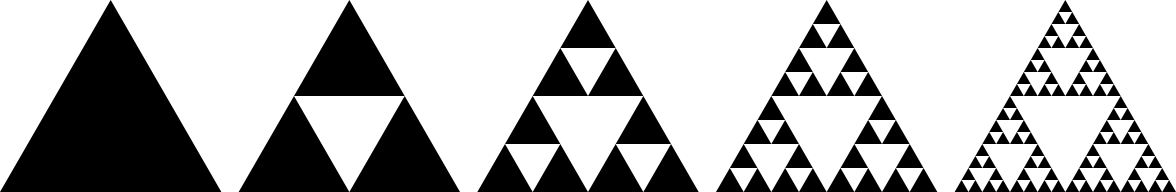
\includegraphics[width=\textwidth]{imgs/Sierpinski_triangle_evolution.png}
%%   \caption{Premières étapes de la construction du triangle équilatéral de Serpienski.}
%%   \label{fig: serpienski triangle}
%% \end{figure}

%% \bigskip
%% \question[5] \textbf{Réduction sur la variété centrale}
%%   \noaddpoints

%%   Considérons le système à temps discret suivant
%%   %
%%   \[
%%     \begin{pmatrix} x \\ y \end{pmatrix}
%%       \mapsto
%%       \begin{pmatrix}
%%         0 & 1 \\
%%         -\nicefrac{1}{2} & \nicefrac{3}{2}
%%       \end{pmatrix}
%%       \begin{pmatrix} x \\ y \end{pmatrix}
%%         +
%%       \begin{pmatrix} 0 \\ -y^3 \end{pmatrix}.
%%   \]

%%   \bigskip

%%   \begin{parts}
%%       \noaddpoints
%%       \part[1] Linéarisez le système autour du point fixe \( (x, y) = (0, 0) \) et calculer les valeurs propres de la matrice Jacobienne. Que pouvez-vous en conclure quant aux propriétés de stabilité de l'origine?

%%       \noaddpoints
%%       \part[1] La matrice \( \bm{V} \) des vecteurs propres et son inverse \( \bm{V}^{-1} \) sont données par
%%       %
%%       \[
%%         \bm{V} =  \begin{bmatrix}
%%                     1 & 2 \\
%%                     1 & 1
%%                   \end{bmatrix}
%%         \quad
%%         \text{et}
%%         \quad
%%         \bm{V}^{-1} =  \begin{bmatrix}
%%                     -1 & 2 \\
%%                     1 & -1
%%                   \end{bmatrix}.
%%       \]
%%       En posant
%%       %
%%       \[
%%         \begin{pmatrix} x \\ y \end{pmatrix}
%%           = \bm{V} \begin{pmatrix} u \\ v \end{pmatrix},
%%       \]
%%       %
%%       donnez les équations gouvernant la dynamique de \( u \) et \( v \).

%%       \noaddpoints
%%       \part[2] Afin de pleinement caractériser la stabilité de l'origine, on cherche la variété centrale
%%       %
%%       \[
%%         W^c(0) = \left\{ (u, v) \vert v = h(u) ; h(0) = Dh(0) = 0 \right\}
%%       \]
%%       %
%%       pour \( u \) suffisament petit.
%%       En supposant que
%%       %
%%       \[
%%         h(u) = a u^2 + b u^3,
%%       \]
%%       %
%%       exprimer l'évolution du système sous la forme \( u \mapsto f(u) \).

%%       \noaddpoints
%%       \part[1] Qu'en concluez vous quant à la stabilité du point fixe à l'origine?
%%   \end{parts}

%%   \addpoints

%%   \question[10] \textbf{Portraits de phase}

%%   \medskip

%%   Pour chacun des systèmes suivants, déterminez les points fixes et leur stabilité (valeurs propres et vecteurs propres).
%%   Ensuite, tracez qualitativement un portrait de phase en faisant explicitement apparaître les points fixes, leurs directions stables et/ou instables, les isoclines ainsi que quelques trajectoires plausibles.

%%   \begin{parts}
%%       \noaddpoints
%%       \part[2] \( \dot{x} = x - y, \quad \dot{y} = 1 - e^x \)
%%       \part[2] \( \dot{x} = x(x-y), \quad \dot{y} = y(2x - y) \)
%%       \part[2] \( \dot{x} = x(2-x-y), \quad \dot{y} = x - y \)
%%       \part[2] \( \dot{x} = x - x^3, \quad \dot{y} = -y \)
%%       \part[2] \( \dot{x} = y, \quad \dot{y} = x(1 + y) - 1 \)
%%   \end{parts}

%%   \addpoints

  % \question[10] \textbf{Théorie de Koopman}
  %
  % \medskip
  %
  % Soit le système dynamique non-linéaire suivant
  % \begin{equation}
  %   \begin{aligned}
  %     \dot{x}_1 & = \mu x_1 \\
  %     \dot{x}_2 & = \lambda \left( x_2 - x_1^4 + 2 x_1^2 \right),
  %   \end{aligned}
  %   \label{eq: exercise 1}
  % \end{equation}
  % avec $\mu < 0$ et $\lambda < 0$.
  %
  %
  % \begin{parts}
  %   % -----> Points fixes et stabilité linéaire.
  %   \noaddpoints
  %   \part[2] Calculez le(s) point(s) fixe(s) du système et étudiez leur stabilité linéaire.
  %
  %   % -----> Variété stable.
  %   \noaddpoints
  %   \part[4] Donnez l'expression des variétés stables du point fixe situé à l'origine et tracer un schéma de l'espace des phases ainsi que quelques trajectoires.
  %
  %   % -----> Théorie de Koopman.
  %   \noaddpoints
  %   \part[4] En introduisant de nouvelles variables, montrez que le système non-linéaire \eqref{eq: exercise 1} peut être ré-écrit sous la forme d'un système linéaire à 4 degrés de liberté.
  %
  %   % -----> Bonus
  %   \noaddpoints
  %   \part[5 Bonus] Calculez les valeurs propres et vecteurs propres du système linéaire obtenu à la question précédente. Concluez quant aux fonctions propres de l'opérateur de Koopman.
  %
  % \end{parts}

\end{questions}

\end{document}
